\documentclass[border=4pt]{standalone}
\usepackage{tikz}
\begin{document}

\noindent
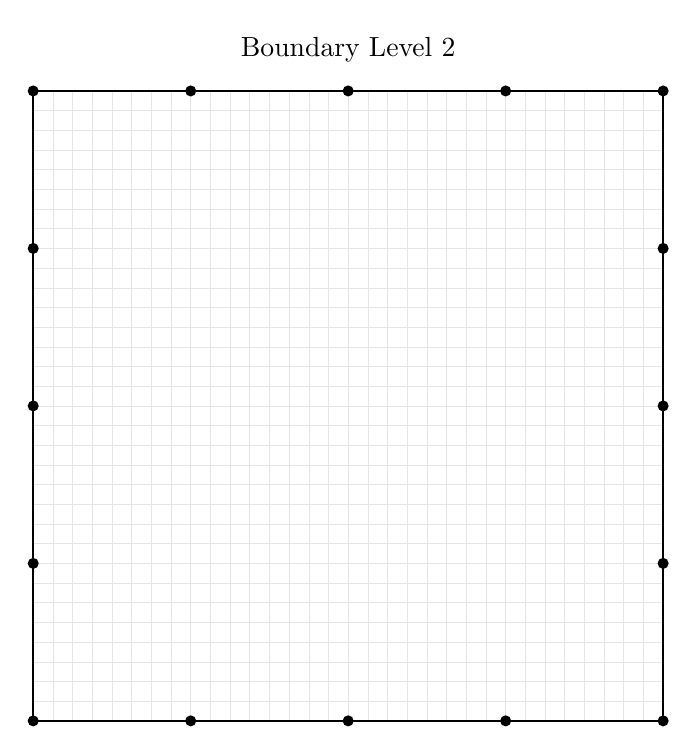
\begin{tikzpicture}[x=0.25cm,y=0.25cm]
  \draw[step=1,black!10,very thin] (0.0,0.0) grid (32.0,32.0);
  \draw[thick] (0,0) rectangle (32,32);
  \node (TOPL) at (16,33) [above,align=center]  {Boundary Level 2};

%% (let* ((p 5)
%%        (m (expt 2 p))
%%        (s 8)
%%        (n (/ m s)))
%%   (cl-loop for x from 0 upto n
%%            do (cl-loop for y from 0 upto n
%%                        when (or (zerop x) (zerop y) (= n x) (= n y))
%%                        do (insert (format "\\fill (%d,%d) circle(2pt);\n" (* s x) (* s y))))))

\fill (0,0) circle(2pt);
\fill (0,8) circle(2pt);
\fill (0,16) circle(2pt);
\fill (0,24) circle(2pt);
\fill (0,32) circle(2pt);
\fill (8,0) circle(2pt);
\fill (8,32) circle(2pt);
\fill (16,0) circle(2pt);
\fill (16,32) circle(2pt);
\fill (24,0) circle(2pt);
\fill (24,32) circle(2pt);
\fill (32,0) circle(2pt);
\fill (32,8) circle(2pt);
\fill (32,16) circle(2pt);
\fill (32,24) circle(2pt);
\fill (32,32) circle(2pt);

\end{tikzpicture}

\end{document}




